
\begin{filecontents*}{example.eps}

gsave
newpath
  20 20 moveto
  20 220 lineto
  220 220 lineto
  220 20 lineto
closepath
2 setlinewidth
gsave
  .4 setgray fill
grestore
stroke
grestore
\end{filecontents*}
%
\RequirePackage{fix-cm}
%
%\documentclass{svjour3}                     % onecolumn (standard format)
%\documentclass[smallcondensed]{svjour3}     % onecolumn (ditto)
\documentclass[smallextended]{svjour3}       % onecolumn (second format)
%\documentclass[twocolumn]{svjour3}          % twocolumn
%
\smartqed  % flush right qed marks, e.g. at end of proof
%
\usepackage{graphicx}
\usepackage{cite}
\usepackage[a4paper]{geometry}

\begin{document}

\title{Google Play Store Analysis}%\thanks{Grants or other notes
%about the article that should go on the front page should be
%placed here. General acknowledgments should be placed at the end of the article.}

%\subtitle{Do you have a subtitle?\\ If so, write it here}

%\titlerunning{Short form of title}        % if too long for running head

\author{Khosh Raftar Nouri, Aida        \and
        Salcedo, Carlos \and
Sarker, Sourav \and
Yazdanpanah, Fatemeh} %etc.
%}

%\authorrunning{Short form of author list} % if too long for running head

\institute{akhoshraftar@mun.ca\\
             cdsalcedo@mun.ca \\
              souravs@mun.ca\\
              fyazdanpanah@mun.ca\\
                       %  \\
%             \emph{Present address:} of F. Author  %  if needed
    %       \and
        %   S. Author \at
            %  second address
}

\date{Received: date / Accepted: date}
% The correct dates will be entered by the editor


\maketitle


\section*{Introduction to data}

While many public datasets (on Kaggle and the like) provide Apple App Store data, there are not many counterpart datasets available for Google Play Store apps anywhere on the web.On digging deeper, it can be found out that iTunes App Store page deploys a nicely indexed appendix-like structure to allow for simple and easy web scraping. On the other hand, Google Play Store uses sophisticated modern-day techniques (like dynamic page load) using JQuery making scraping more challenging.
The Play Store apps data has enormous potential to drive app-making businesses to success. Actionable insights can be drawn for developers to work on and capture the Android market!
Each app (row) has values for catergory, rating, reviews, size, installs, price, rated, last updated, and version.


\section*{Objectives of Google-Play Store Analysis}
This project focuses on the analysis of the Play Store data set in Kaggle.
The aim of this project is:
\begin{itemize}
\item Using the data to analyze consumer trends and determine which type of apps are the most popular and profitable.\\
\item Classifying applications based on their categories.\\
\item Presenting the growth of applications from 2016 to 2018.\\
\item Comparing different categories of applications based on the Android version.\\
\item Comparing the rates in different kinds of applications.\\
\item Assessing supported Android version with numbers of reviews based on different categories.\\
\end{itemize}

\section*{Categories of Applications}
In our dataset we have more than 9000 applications. The pie chart represents top 20 application categories based on application number. (Figure 1)
\begin{itemize}
\item
  Family is included of 1832  numbers of applications.
\item
  Game is included of 959  numbers of applications.
  \item
  Tools is included of 827  numbers of applications.
\item
  Business is included of 420  numbers of applications.
\item
  Medicul is included of 395  numbers of applications.
\end{itemize}

This result shows that the major numbers of applications is related to Family.
\begin{figure}
\centering
\includegraphics[width=7cm,height=7cm]{pic/pie_chart}
\caption{Top 20 Application Categories Based on Application Number}
\label{fig:1}
\end{figure}

\section*{Growth of Application Numbers from 2016-2018}
According to bar chart, (Figure 2), we can see the growth of application numbers which are categorized in different years. Most of the applications have grown in all three years from 2016-2018.
Family reached to the top of growth around 200, 400, and 800 in 2016, 2017, and 2018 respectively. The following highest application number in all three years are belonged to Tools and Business.

\begin{figure}
\centering
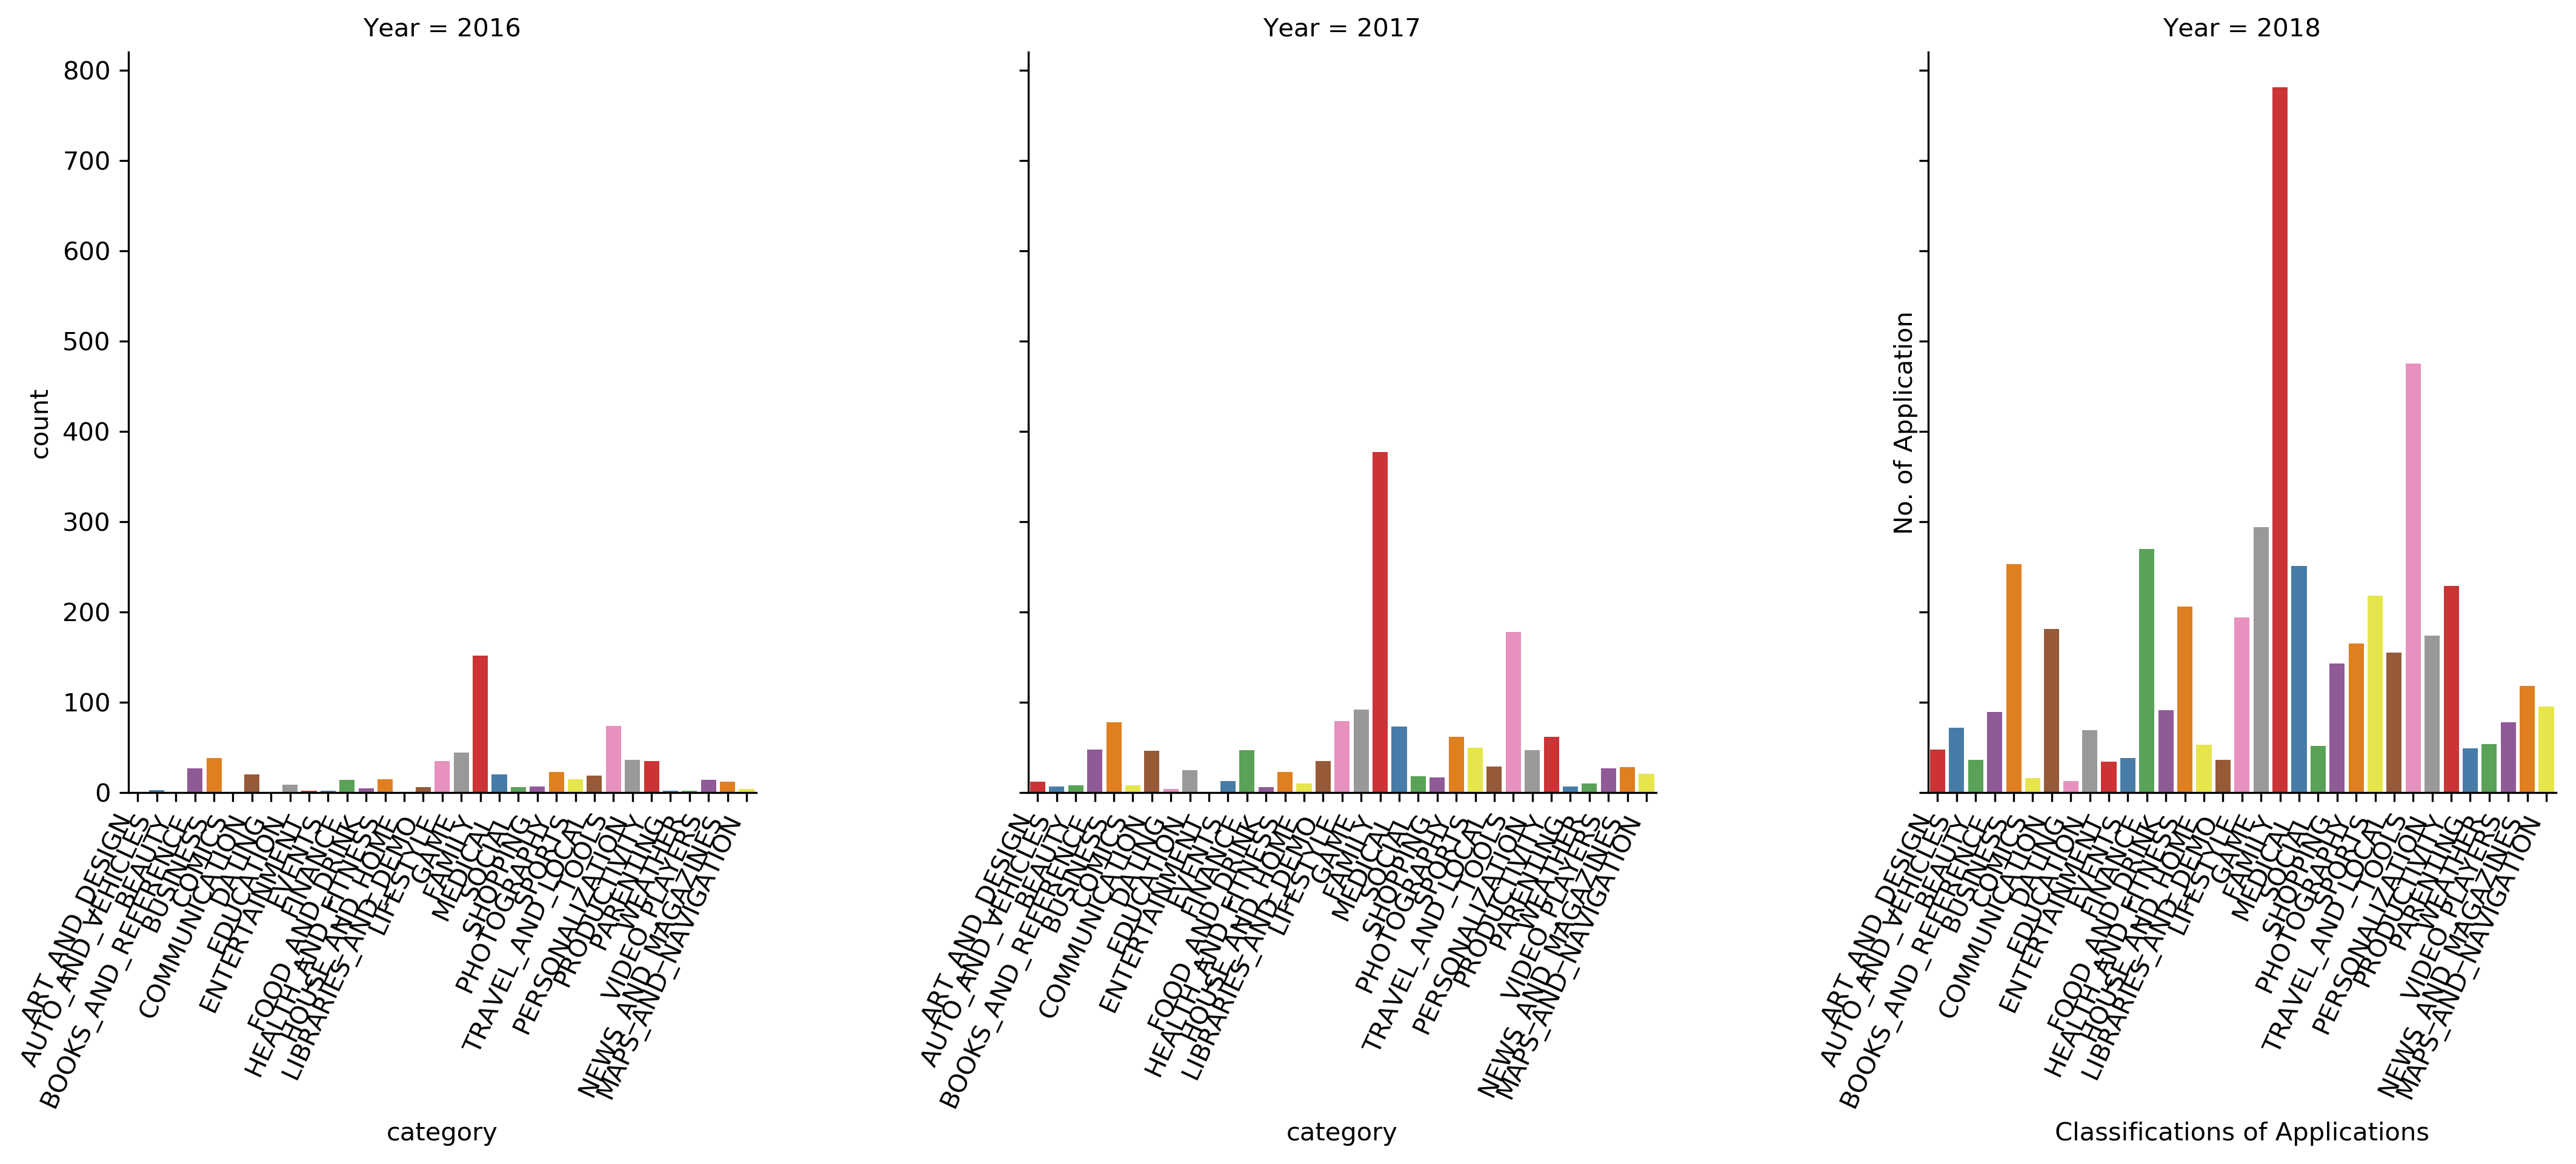
\includegraphics[width=15cm,height=7cm]{pic/cat_plot}
\caption{Gnre (Everyone) vs No. of Application Got Updated in 2018} 
\label{fig:2}
\end{figure}	

\section*{update}
\subsection*{Number of Application Update}
From the survey carried out, Family, Tools, and Business have the most updated numbers of applications which reaches around 800 in 2018. While, Dating and Comics have less updated compared to others. (Figure 3)  
\begin{figure}
\centering
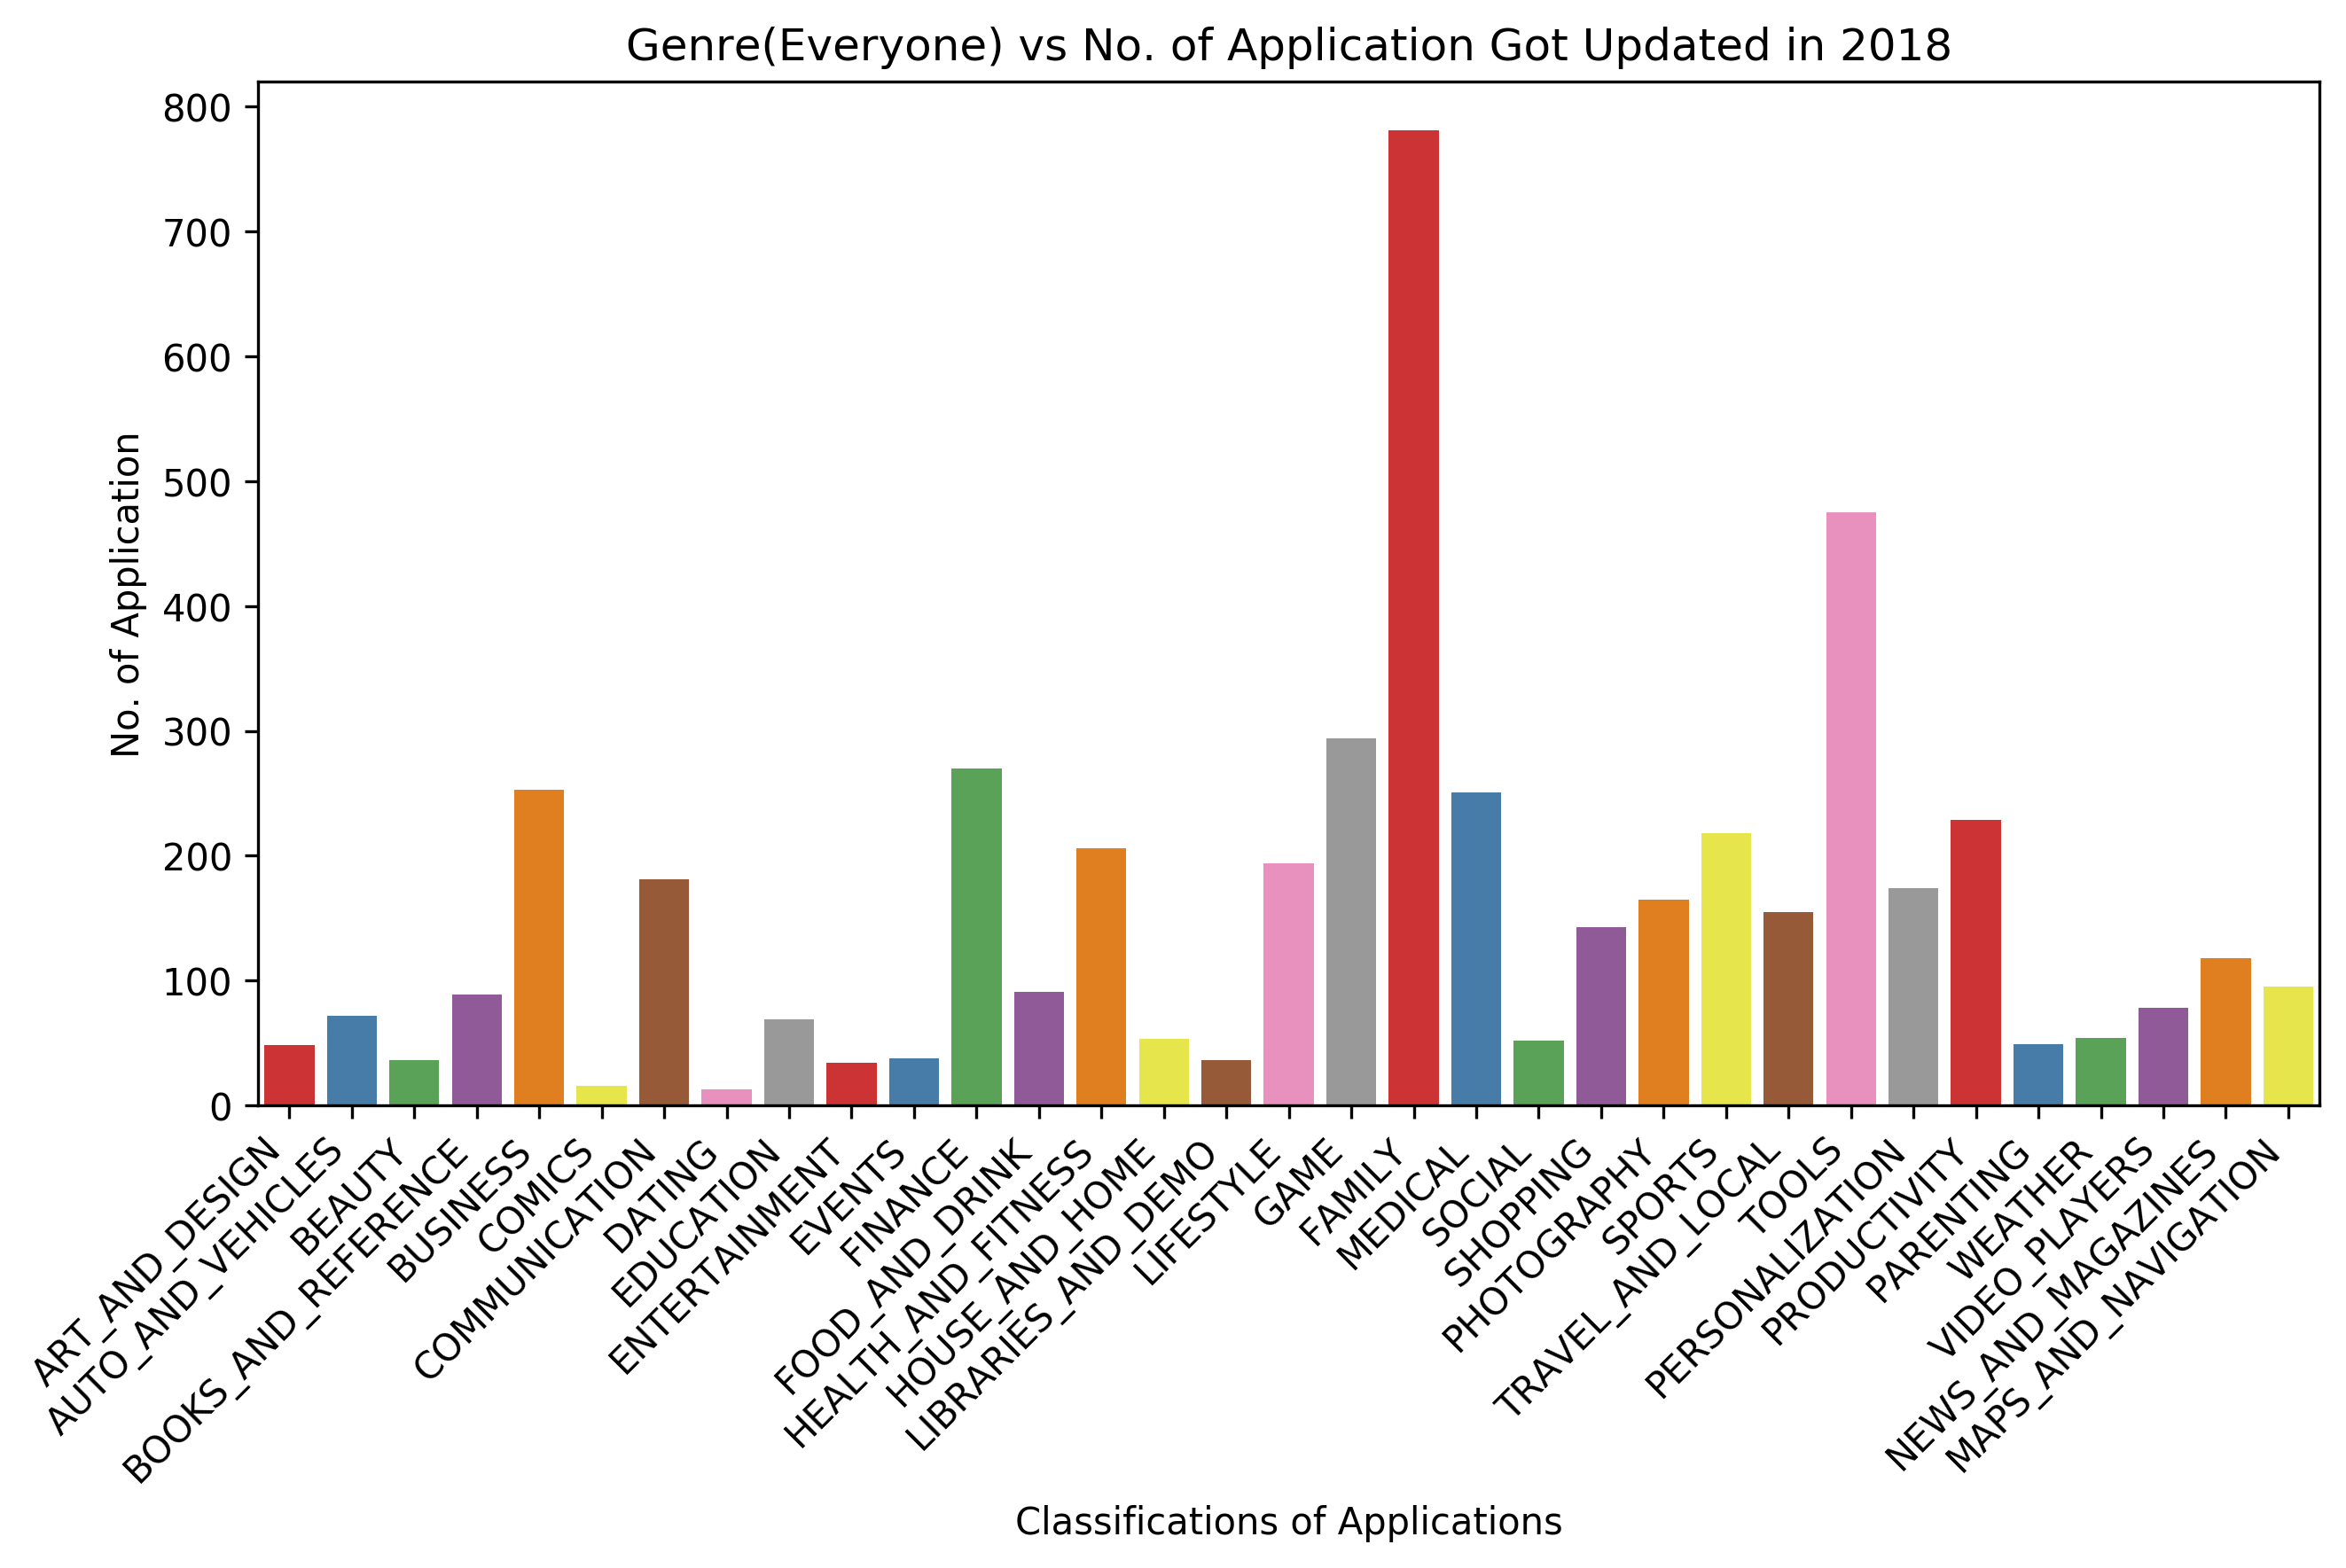
\includegraphics[width=10cm,height=10cm]{pic/counter_plot}
\caption{... }
\label{fig:3}
\end{figure}

\subsection*{Different Months of Application Update}
This figure represents the update of application based on the differences between months and years. The highest rate of update is belonged to month of July in 2018. As shown in Figure 3, in 2018, there is a great trend of update compared to other years. (Figure 4)
\begin{figure}
\centering
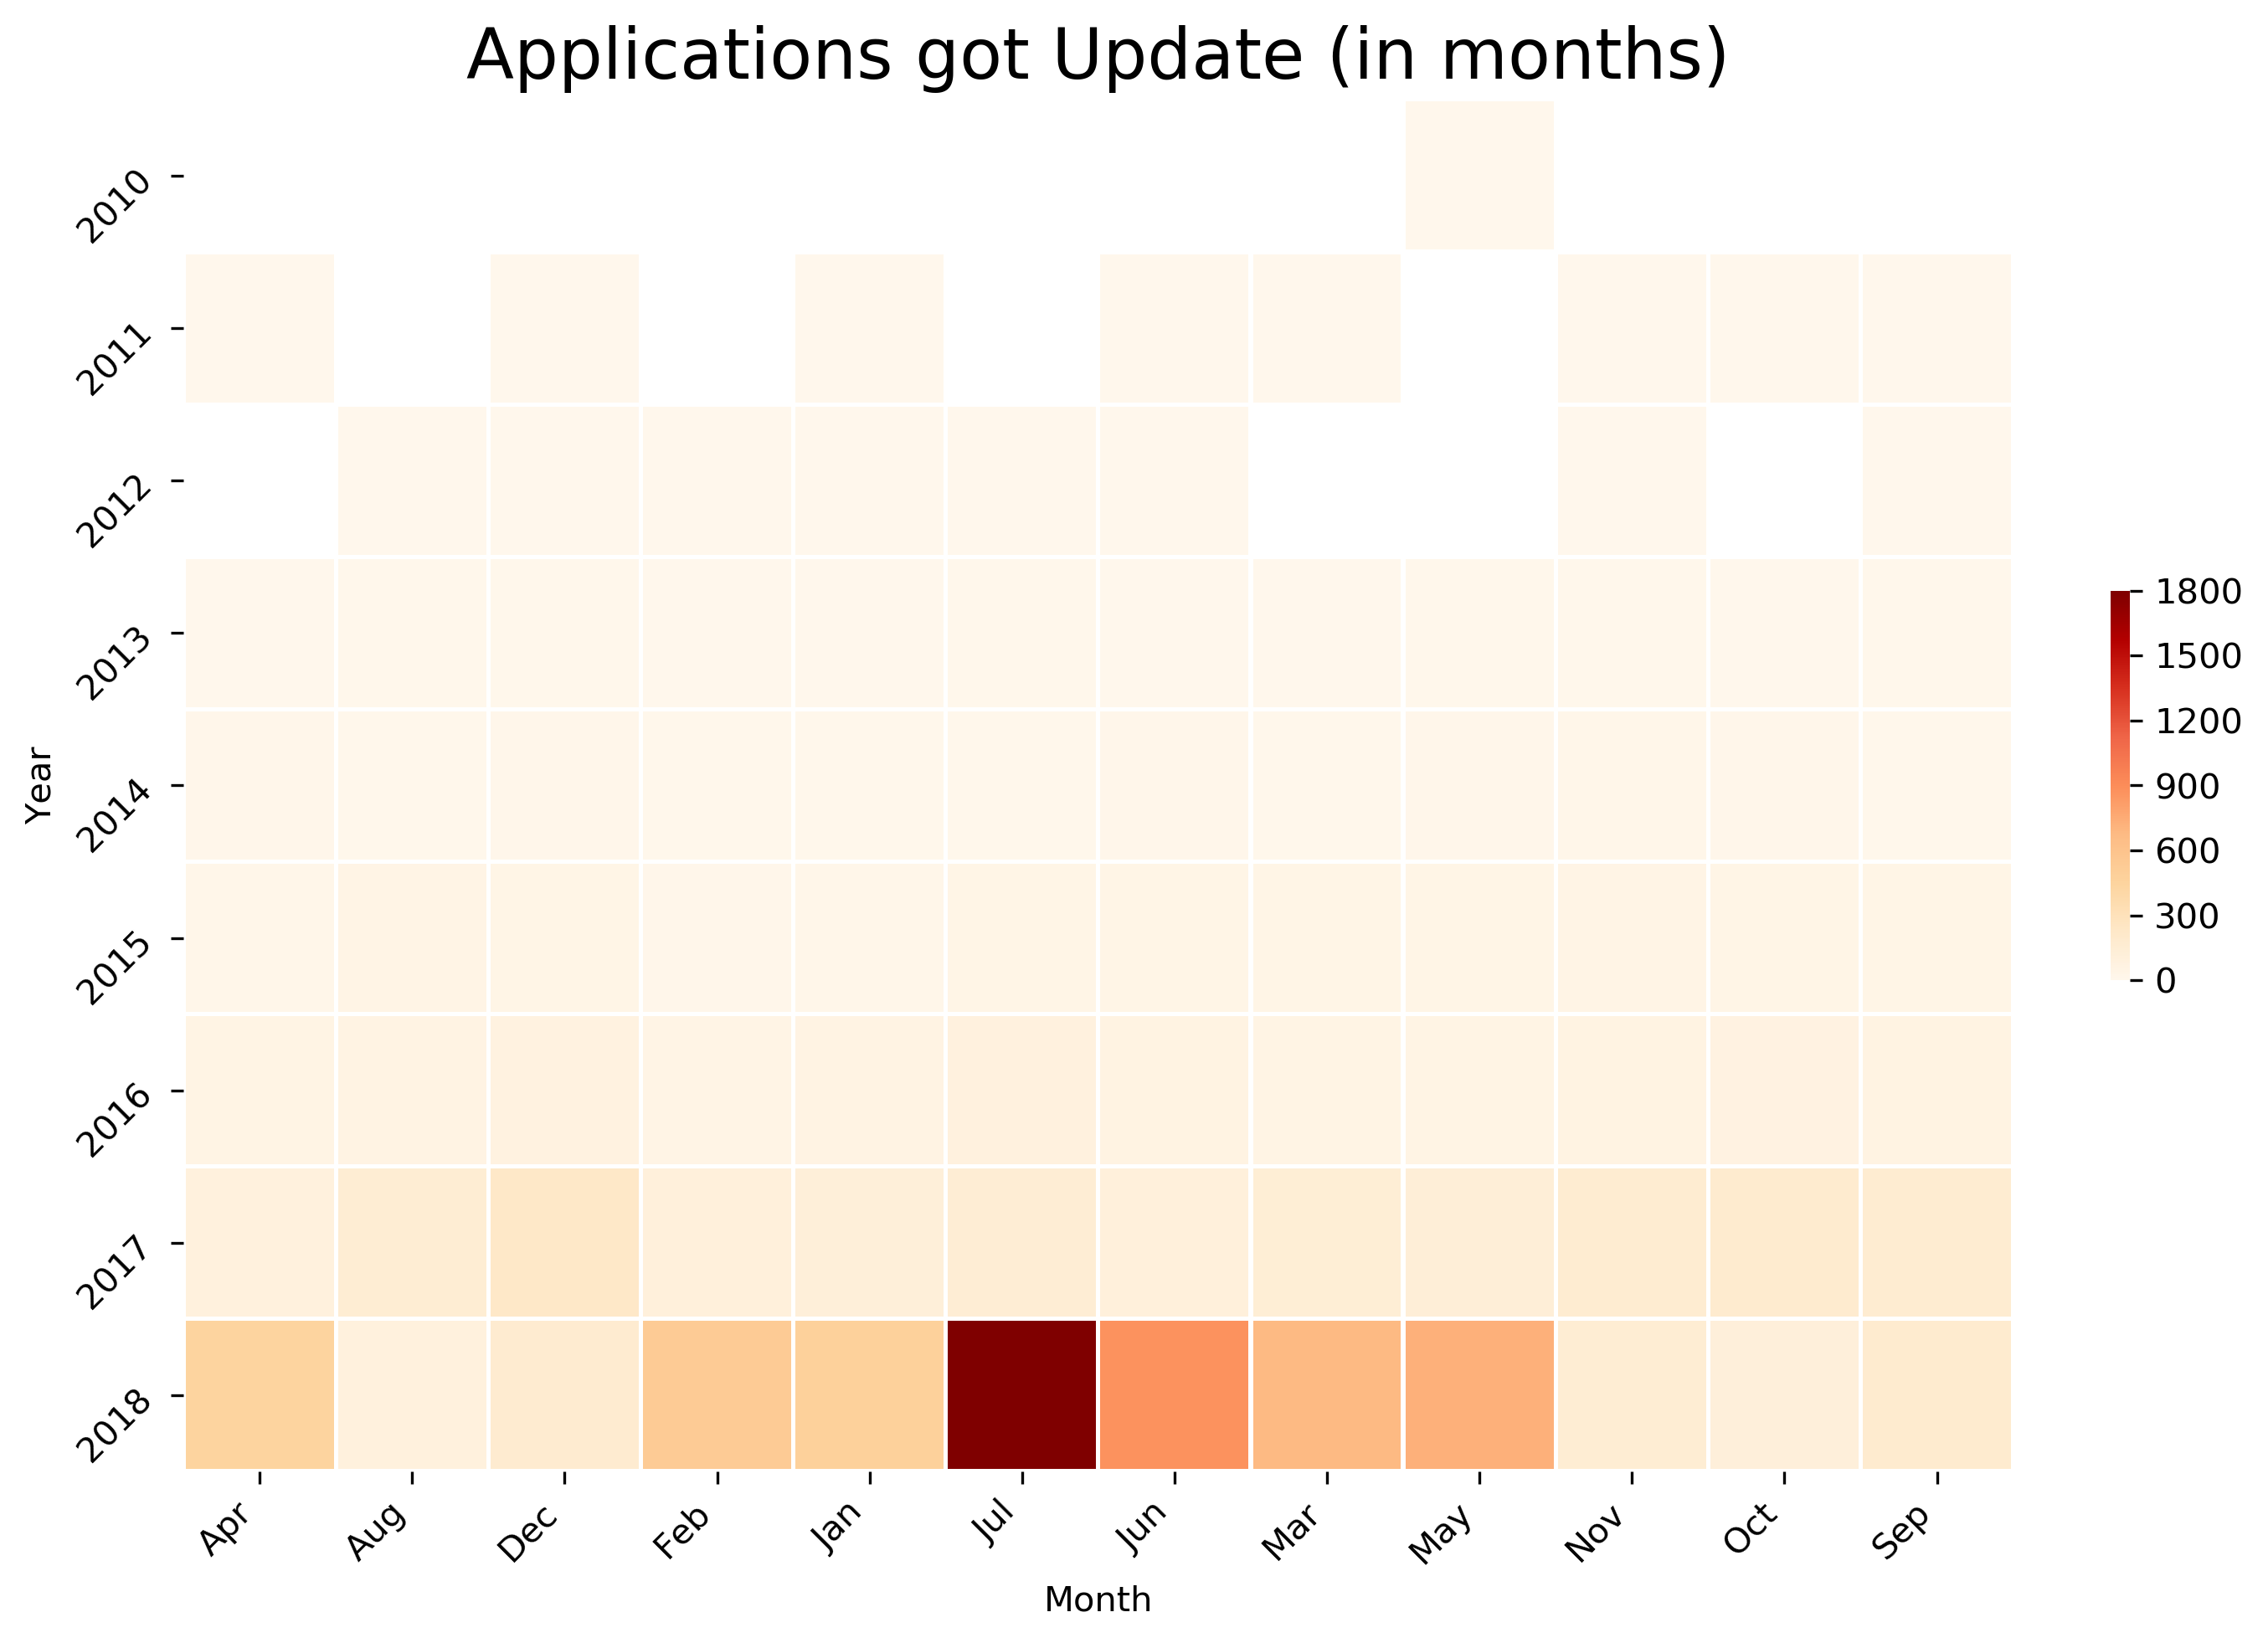
\includegraphics[width=10cm,height=10cm]{pic/heatmap_2}
\caption{... }
\label{fig:4}
\end{figure}

\section*{Android Version}
\subsection*{Supported Android Version with No. reviews based on Game}
This graph describes the supported Android version with number of reviews based on game.
\begin{itemize}
\item The majority number of reviews are belonged to version of 4.1, 4.0.3, 2.3, 4.0, 4.4 and up.\\
\item Among Everyone (orange dot) and Teen (red dot), 4.1,4.0.3, and 2.3 are seen significantly.\\
\item Some versions which are less than two have no review as shown in the figure.\\
\end{itemize}

\begin{figure}
\centering
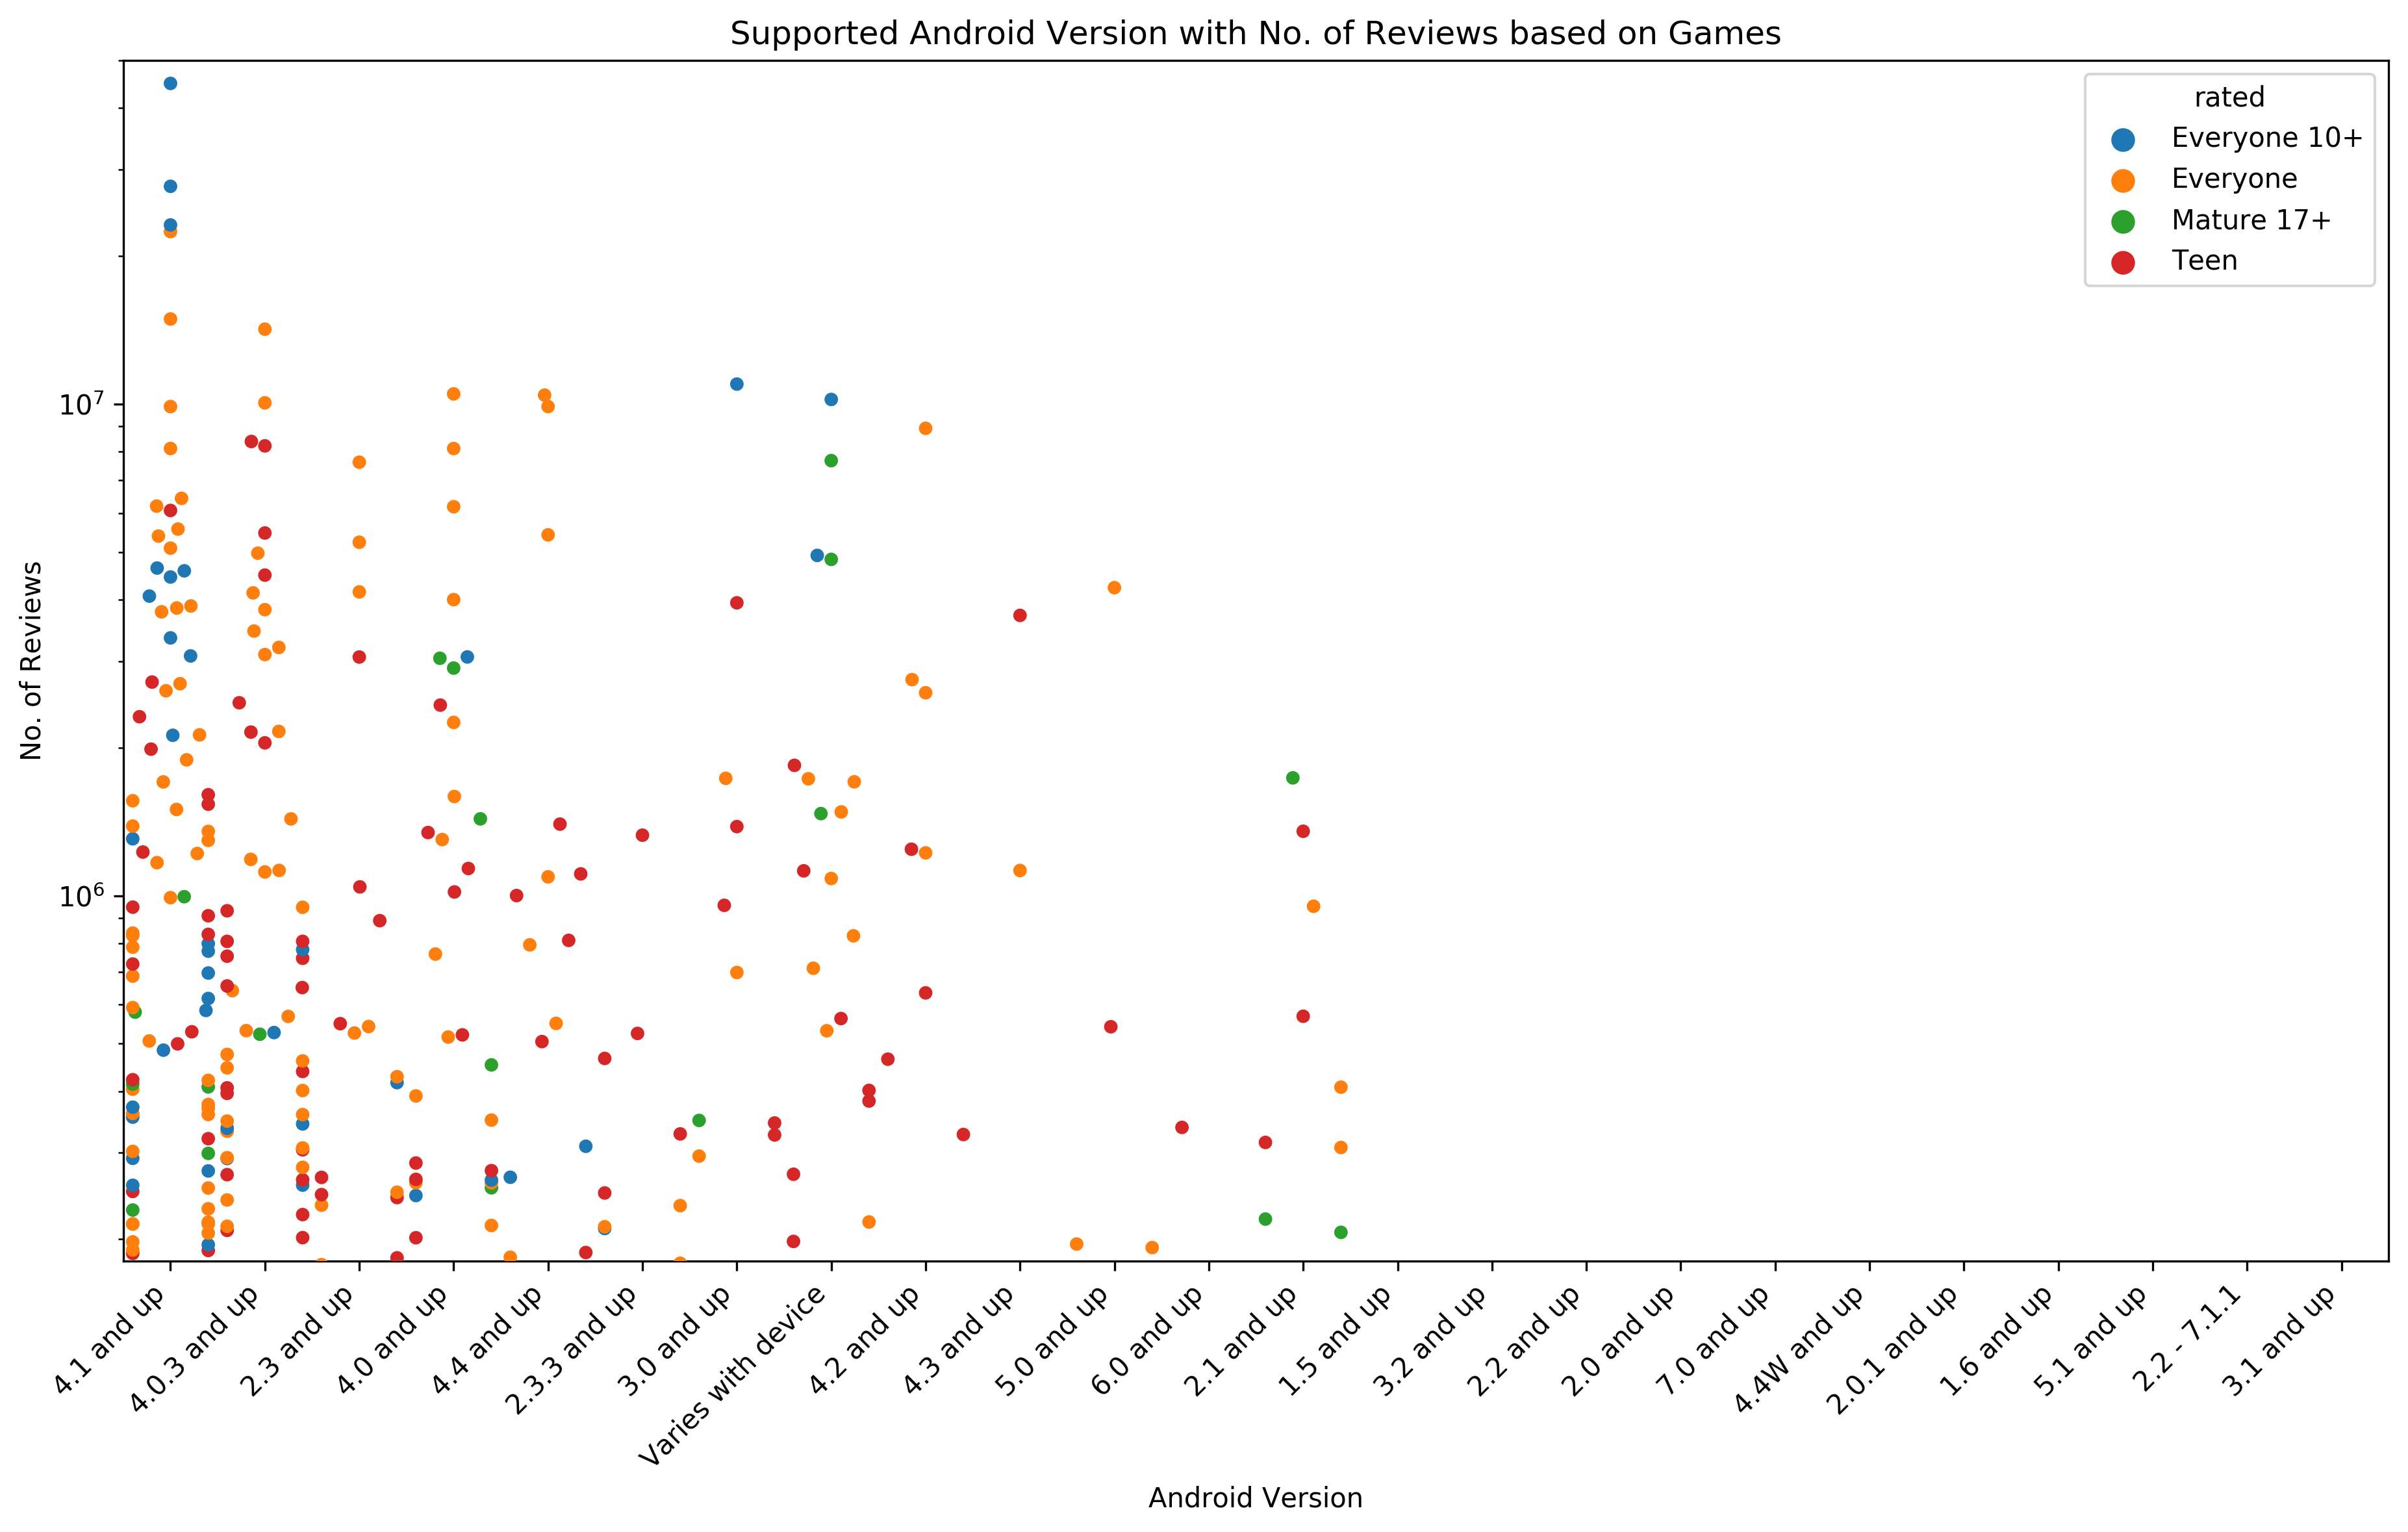
\includegraphics[width=10cm,height=10cm]{pic/swarm_plot}
\caption{Supported Android Version with No. reviews based on Game}
\label{fig:5}
\end{figure}

\end{document}
% end of file template.tex

